% Options for packages loaded elsewhere
\PassOptionsToPackage{unicode}{hyperref}
\PassOptionsToPackage{hyphens}{url}
%
\documentclass[
  12pt,
]{article}
\usepackage{amsmath,amssymb}
\usepackage{lmodern}
\usepackage{iftex}
\ifPDFTeX
  \usepackage[T1]{fontenc}
  \usepackage[utf8]{inputenc}
  \usepackage{textcomp} % provide euro and other symbols
\else % if luatex or xetex
  \usepackage{unicode-math}
  \defaultfontfeatures{Scale=MatchLowercase}
  \defaultfontfeatures[\rmfamily]{Ligatures=TeX,Scale=1}
\fi
% Use upquote if available, for straight quotes in verbatim environments
\IfFileExists{upquote.sty}{\usepackage{upquote}}{}
\IfFileExists{microtype.sty}{% use microtype if available
  \usepackage[]{microtype}
  \UseMicrotypeSet[protrusion]{basicmath} % disable protrusion for tt fonts
}{}
\makeatletter
\@ifundefined{KOMAClassName}{% if non-KOMA class
  \IfFileExists{parskip.sty}{%
    \usepackage{parskip}
  }{% else
    \setlength{\parindent}{0pt}
    \setlength{\parskip}{6pt plus 2pt minus 1pt}}
}{% if KOMA class
  \KOMAoptions{parskip=half}}
\makeatother
\usepackage{xcolor}
\IfFileExists{xurl.sty}{\usepackage{xurl}}{} % add URL line breaks if available
\IfFileExists{bookmark.sty}{\usepackage{bookmark}}{\usepackage{hyperref}}
\hypersetup{
  pdftitle={Reporte del Reto - Análisis de SARS-CoV-2},
  pdfauthor={Anette Pamela Ruiz Abreu, Antonio Noguerón Bárcenas \& Patricio Álvarez Hernández},
  hidelinks,
  pdfcreator={LaTeX via pandoc}}
\urlstyle{same} % disable monospaced font for URLs
\usepackage[margin=1in]{geometry}
\usepackage{color}
\usepackage{fancyvrb}
\newcommand{\VerbBar}{|}
\newcommand{\VERB}{\Verb[commandchars=\\\{\}]}
\DefineVerbatimEnvironment{Highlighting}{Verbatim}{commandchars=\\\{\}}
% Add ',fontsize=\small' for more characters per line
\usepackage{framed}
\definecolor{shadecolor}{RGB}{248,248,248}
\newenvironment{Shaded}{\begin{snugshade}}{\end{snugshade}}
\newcommand{\AlertTok}[1]{\textcolor[rgb]{0.94,0.16,0.16}{#1}}
\newcommand{\AnnotationTok}[1]{\textcolor[rgb]{0.56,0.35,0.01}{\textbf{\textit{#1}}}}
\newcommand{\AttributeTok}[1]{\textcolor[rgb]{0.77,0.63,0.00}{#1}}
\newcommand{\BaseNTok}[1]{\textcolor[rgb]{0.00,0.00,0.81}{#1}}
\newcommand{\BuiltInTok}[1]{#1}
\newcommand{\CharTok}[1]{\textcolor[rgb]{0.31,0.60,0.02}{#1}}
\newcommand{\CommentTok}[1]{\textcolor[rgb]{0.56,0.35,0.01}{\textit{#1}}}
\newcommand{\CommentVarTok}[1]{\textcolor[rgb]{0.56,0.35,0.01}{\textbf{\textit{#1}}}}
\newcommand{\ConstantTok}[1]{\textcolor[rgb]{0.00,0.00,0.00}{#1}}
\newcommand{\ControlFlowTok}[1]{\textcolor[rgb]{0.13,0.29,0.53}{\textbf{#1}}}
\newcommand{\DataTypeTok}[1]{\textcolor[rgb]{0.13,0.29,0.53}{#1}}
\newcommand{\DecValTok}[1]{\textcolor[rgb]{0.00,0.00,0.81}{#1}}
\newcommand{\DocumentationTok}[1]{\textcolor[rgb]{0.56,0.35,0.01}{\textbf{\textit{#1}}}}
\newcommand{\ErrorTok}[1]{\textcolor[rgb]{0.64,0.00,0.00}{\textbf{#1}}}
\newcommand{\ExtensionTok}[1]{#1}
\newcommand{\FloatTok}[1]{\textcolor[rgb]{0.00,0.00,0.81}{#1}}
\newcommand{\FunctionTok}[1]{\textcolor[rgb]{0.00,0.00,0.00}{#1}}
\newcommand{\ImportTok}[1]{#1}
\newcommand{\InformationTok}[1]{\textcolor[rgb]{0.56,0.35,0.01}{\textbf{\textit{#1}}}}
\newcommand{\KeywordTok}[1]{\textcolor[rgb]{0.13,0.29,0.53}{\textbf{#1}}}
\newcommand{\NormalTok}[1]{#1}
\newcommand{\OperatorTok}[1]{\textcolor[rgb]{0.81,0.36,0.00}{\textbf{#1}}}
\newcommand{\OtherTok}[1]{\textcolor[rgb]{0.56,0.35,0.01}{#1}}
\newcommand{\PreprocessorTok}[1]{\textcolor[rgb]{0.56,0.35,0.01}{\textit{#1}}}
\newcommand{\RegionMarkerTok}[1]{#1}
\newcommand{\SpecialCharTok}[1]{\textcolor[rgb]{0.00,0.00,0.00}{#1}}
\newcommand{\SpecialStringTok}[1]{\textcolor[rgb]{0.31,0.60,0.02}{#1}}
\newcommand{\StringTok}[1]{\textcolor[rgb]{0.31,0.60,0.02}{#1}}
\newcommand{\VariableTok}[1]{\textcolor[rgb]{0.00,0.00,0.00}{#1}}
\newcommand{\VerbatimStringTok}[1]{\textcolor[rgb]{0.31,0.60,0.02}{#1}}
\newcommand{\WarningTok}[1]{\textcolor[rgb]{0.56,0.35,0.01}{\textbf{\textit{#1}}}}
\usepackage{graphicx}
\makeatletter
\def\maxwidth{\ifdim\Gin@nat@width>\linewidth\linewidth\else\Gin@nat@width\fi}
\def\maxheight{\ifdim\Gin@nat@height>\textheight\textheight\else\Gin@nat@height\fi}
\makeatother
% Scale images if necessary, so that they will not overflow the page
% margins by default, and it is still possible to overwrite the defaults
% using explicit options in \includegraphics[width, height, ...]{}
\setkeys{Gin}{width=\maxwidth,height=\maxheight,keepaspectratio}
% Set default figure placement to htbp
\makeatletter
\def\fps@figure{htbp}
\makeatother
\setlength{\emergencystretch}{3em} % prevent overfull lines
\providecommand{\tightlist}{%
  \setlength{\itemsep}{0pt}\setlength{\parskip}{0pt}}
\setcounter{secnumdepth}{-\maxdimen} % remove section numbering
\ifLuaTeX
  \usepackage{selnolig}  % disable illegal ligatures
\fi

\title{Reporte del Reto - Análisis de SARS-CoV-2}
\author{Anette Pamela Ruiz Abreu, Antonio Noguerón Bárcenas \& Patricio
Álvarez Hernández}
\date{4 de mayo de 2022}

\begin{document}
\maketitle

\hypertarget{introducciuxf3n}{%
\subsubsection{Introducción:}\label{introducciuxf3n}}

A finales de 2019 la ciudad de Wuhan, en la provincia de Hubei (una
ciudad de China con más de 11 millones de habitantes), se convirtió en
el centro de una epidemia de neumonía de causa desconocida con
implicaciones globales.

En enero de 2020, la Organización Mundial de la Salud (OMS) declaró el
brote de la enfermedad por el nuevo coronavirus SARS-CoV-2 (COVID-19)
como una emergencia de salud pública de importancia internacional. En
marzo de 2020, caracterizó el COVID-19 como una pandemia. Desde entonces
la OMS y las autoridades de salud pública de todo el mundo están
actuando para contener el brote, que ha implicado desafíos antes
impensados para las personas, las comunidades y las instituciones.

Esta pandemia puede ser considerada como el primer gran impacto de
repercusión planetaria en la historia reciente del mundo globalizado.
Aunque sus efectos en materia de salud pública están siendo
superlativos, también lo son en todos los demás ámbitos de la vida
pública y privada, individual y colectiva. Como es el caso en la mayoría
de los procesos naturales, sus oportunidades o contingencias asociadas
dependen del modelo de desarrollo en el que se produzcan. Con la
pandemia, esto se ha puesto más en evidencia.

Se sabe que las pruebas serológicas son una herramienta muy útil para
confirmar la infección por un patógeno en la población y, combinadas con
datos epidemiológicos y clínicos, permiten estimar la gravedad y la
transmisibilidad del patógeno e identificar los grupos de población que
han sido infectados, así como aquellos que siguen siendo susceptibles.
Por ello, cada vez más requerimos datos moleculares como las secuencias
de ácidos nucleicos de los virus para conocer su origen y potencialidad
epidemiológica.

\hypertarget{problema}{%
\subsubsection{Problema:}\label{problema}}

El SARS-CoV-2 es un virus que causa una enfermedad respiratoria llamada
enfermedad por coronavirus de 2019 (COVID-19). El SARS-CoV-2 es un virus
de la gran familia de los coronavirus. Los coronavirus infectan a seres
humanos y algunos animales. La infección por el SARS-CoV-2 en las
personas se identificó por primera vez en 2019. Se piensa que este virus
se transmite de una persona a otra en las gotitas que se dispersan
cuando la persona infectada tose, estornuda o habla. Es posible que
también se transmita por tocar una superficie con el virus y luego
llevarse las manos a la boca, la nariz o los ojos, aunque esto es menos
frecuente. Hay estudios de investigación en curso sobre el tratamiento
de la COVID-19 y la prevención de la infección por el SARS-CoV-2.
También se llama coronavirus 2019-nCoV, coronavirus del síndrome
respiratorio agudo grave de tipo 2 y CoV-SRAG-2.

Sabemos que un virus al contagiarse y replicarse numerosas veces, tiene
la posibilidad de mutar y generar un cambio en su ADN. A la hora de
hacer el proceso de la replicación, es posible que haya cambios a la
hora de copiar el genoma de los virus de generaciones anteriores. Es
decir, mientras más contagios haya, las posibilidades de tener
mutaciones son mayores y se van distanciando del genoma original, ya sea
para el bien del virus, o del organismo hospedante.

Sabemos que el SARS-CoV-2 es un virus increíblemente contagioso y
peligroso. Un año después de que empezó la pandemia, se empezaron a
crear y distribuir vacunas; sin embargo, el virus no desapareció y la
pandemia persistió gracias a que había personas que no querían vacunarse
o no había suficientes vacunas para la población. El virus empezó a
mutar y se volvió más resistente a las primeras vacunas.

Es gracias a estas mutaciones que han surgido variantes de preocupación
como Delta y Omicrón. Una variante es un código genético que puede tener
una o más mutaciones, y una de preocupación es aquella que puede ser más
transmisible, mortal, y que además, puede poner en riesgo la efectividad
de las herramientas médicas actuales para combatir al virus.

\hypertarget{antecedentes}{%
\subsubsection{Antecedentes:}\label{antecedentes}}

\hypertarget{cronologuxeda-del-covid}{%
\paragraph{\texorpdfstring{\textbf{Cronología del
Covid:}}{Cronología del Covid:}}\label{cronologuxeda-del-covid}}

\hypertarget{de-diciembre-de-2019}{%
\subparagraph{\texorpdfstring{\textbf{31 de diciembre de
2019}}{31 de diciembre de 2019}}\label{de-diciembre-de-2019}}

La Oficina de la OMS en la República Popular China detecta una
declaración de la Comisión Municipal de Salud de Wuhan para los medios
de comunicación publicada en su sitio web en la que se mencionan casos
de una «neumonía vírica» en Wuhan (República Popular China).

\hypertarget{de-enero-de-2020}{%
\subparagraph{\texorpdfstring{\textbf{13 de enero de
2020}}{13 de enero de 2020}}\label{de-enero-de-2020}}

El Ministro de Salud Pública de Tailandia notifica un caso del nuevo
coronavirus confirmado en laboratorio importado desde Wuhan, el primer
caso registrado fuera de la República Popular China.

\hypertarget{de-enero-de-2020-1}{%
\subparagraph{\texorpdfstring{\textbf{16 de enero de
2020}}{16 de enero de 2020}}\label{de-enero-de-2020-1}}

El Ministerio de Salud, Trabajo y Bienestar del Japón notifica a la OMS
un caso confirmado de infección por el nuevo coronavirus en una persona
que había viajado a Wuhan. Es el segundo caso confirmado detectado fuera
de la República Popular China.

\hypertarget{de-enero-de-2020-2}{%
\subparagraph{\texorpdfstring{\textbf{21 de enero de
2020}}{21 de enero de 2020}}\label{de-enero-de-2020-2}}

Los Estados Unidos de América (EE.UU.) notifican su primer caso
confirmado de infección por el nuevo coronavirus. Se trata del primer
caso en la Región de las Américas de la OMS. El hombre había viajado a
Wuhan.

\hypertarget{de-enero-de-2020-3}{%
\subparagraph{\texorpdfstring{\textbf{24 de enero de
2020}}{24 de enero de 2020}}\label{de-enero-de-2020-3}}

Francia notifica a la OMS tres casos de infección por el nuevo
coronavirus, todos de personas que habían viajado desde Wuhan. Se trata
de los primeros casos confirmados en la Región de Europa de la OMS
(EURO).

\hypertarget{de-enero-de-2020-4}{%
\subparagraph{\texorpdfstring{\textbf{29 de enero de
2020}}{29 de enero de 2020}}\label{de-enero-de-2020-4}}

Los Emiratos Árabes Unidos notifican los primeros casos en la Región del
Mediterráneo Oriental.

\hypertarget{de-febrero-de-2022}{%
\subparagraph{\texorpdfstring{\textbf{14 de febrero de
2022}}{14 de febrero de 2022}}\label{de-febrero-de-2022}}

Egipto anuncia su primer caso de coronavirus de Wuhan, según un
comunicado conjunto del Ministerio de Salud de Egipto y la OMS. Es el
primer caso confirmado en África desde que se detectó el virus.

\hypertarget{de-febrero-de-2020}{%
\subparagraph{\texorpdfstring{\textbf{25 de febrero de
2020}}{25 de febrero de 2020}}\label{de-febrero-de-2020}}

Confirmación del primer caso en la Región de África de la OMS, en
Argelia. Este caso llega después de la notificación previa de un caso en
Egipto, el primero en el continente africano. Fue un hombre que había
viajado a Italia.

\hypertarget{de-febrero-de-2020-1}{%
\subparagraph{\texorpdfstring{\textbf{28 de febrero de
2020}}{28 de febrero de 2020}}\label{de-febrero-de-2020-1}}

El primer caso fue detectado en Ciudad de México. Un hombre de 35 años
que había visitado recientemente el norte de Italia.

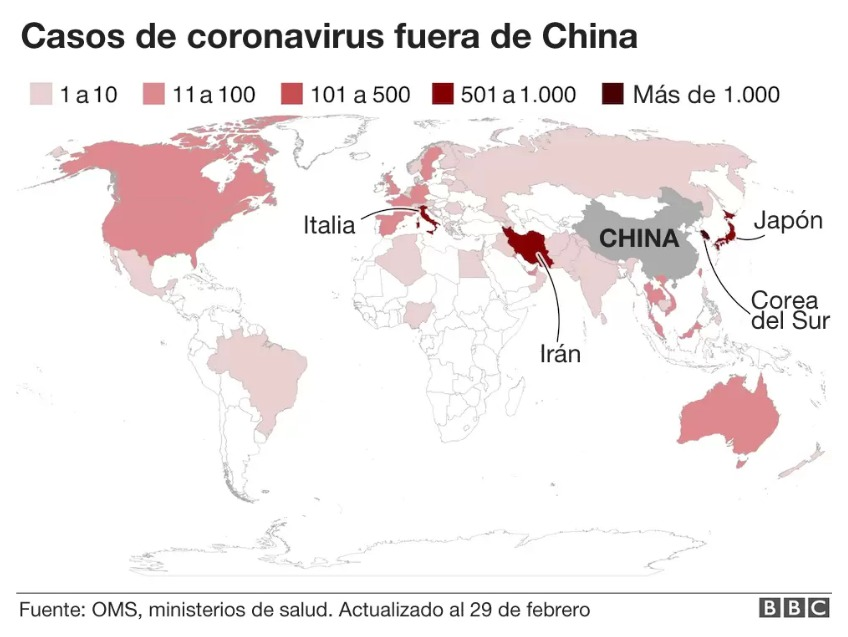
\includegraphics{Archivos/Image1.jpeg}
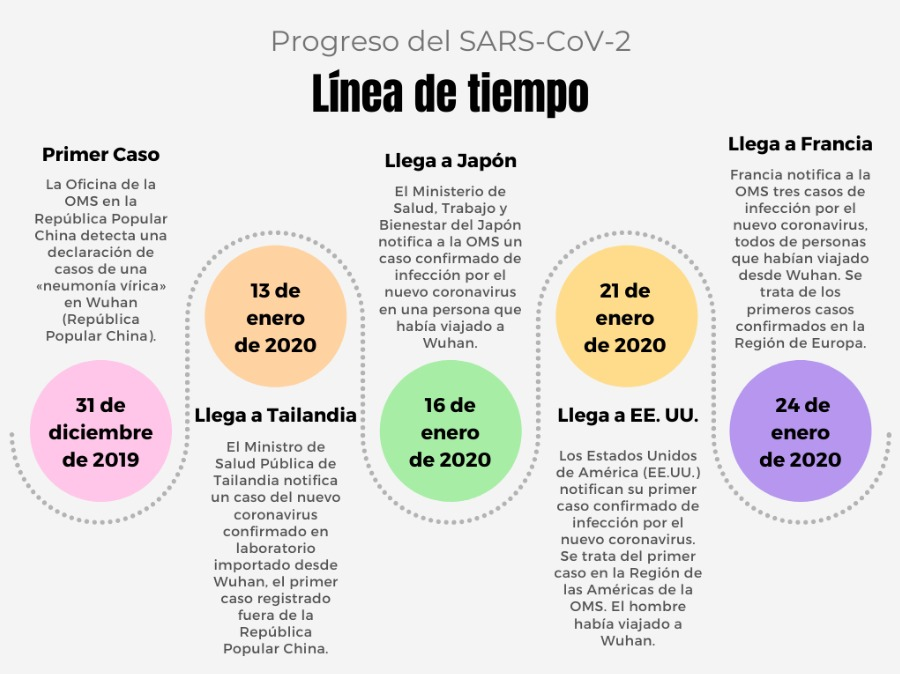
\includegraphics{Archivos/Image2.jpeg}
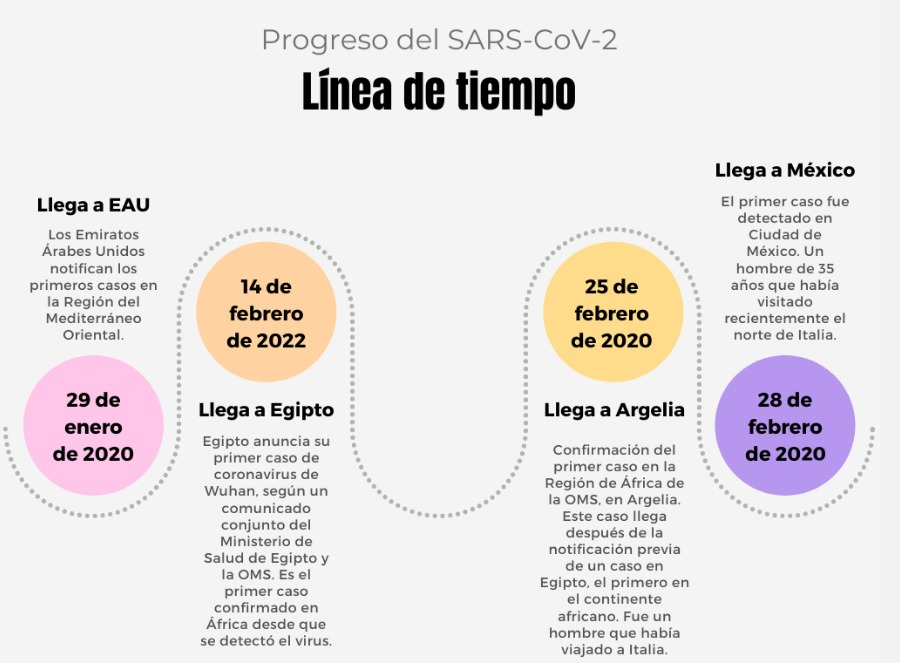
\includegraphics{Archivos/Image3.jpeg}

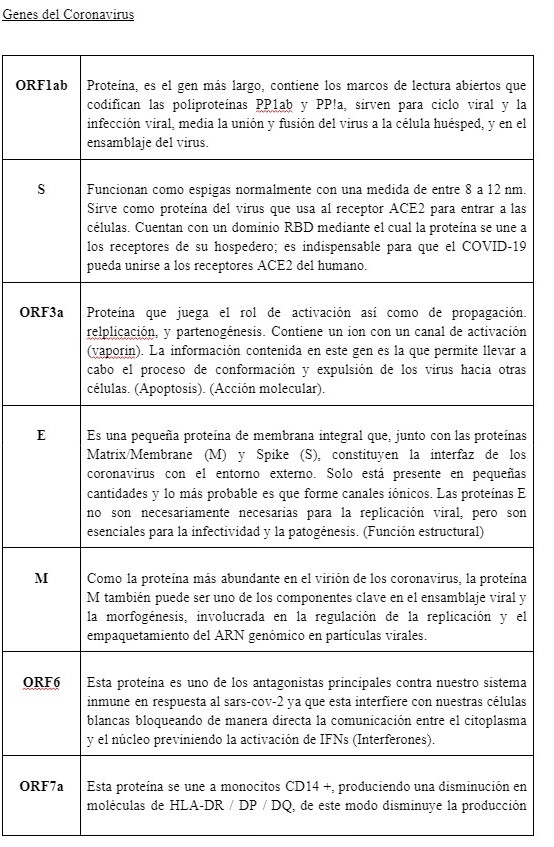
\includegraphics{Archivos/Image5.jpeg}
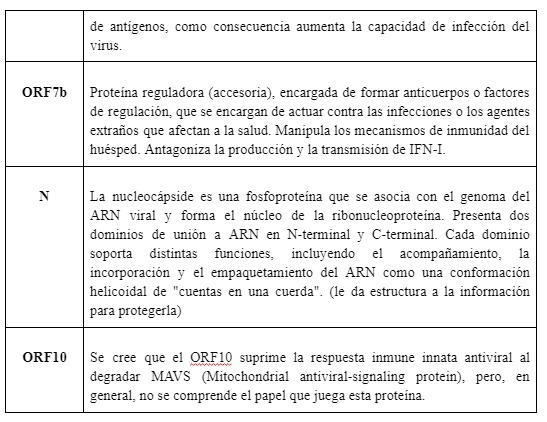
\includegraphics{Archivos/Image6.jpeg}

\hypertarget{propuesta}{%
\subsubsection{Propuesta:}\label{propuesta}}

Analizar el progreso de una de las variantes del SARS-CoV-2 a través del
mundo hasta llegar a México; esto mediante el análisis de las mutaciones
de la variante en distintos genomas recopilados en distintos países. Al
identificar las mutaciones más relevantes y recurrentes, investigar las
repercusiones de las mutaciones y ligarlas con las noticias sobre el
progreso del virus.

\hypertarget{hipuxf3tesis}{%
\subsubsection{Hipótesis:}\label{hipuxf3tesis}}

\hypertarget{hipuxf3tesis-1}{%
\paragraph{Hipótesis 1:}\label{hipuxf3tesis-1}}

El virus original del SARS-CoV-2 de Wuhan no sufrió ninguna mutación en
sus genes más importantes (S, E, M, N) al propagarse a los siguientes
países de interés: Estados Unidos, México, Italia, Japón, Tailandia y
Francia.

\hypertarget{hipuxf3tesis-2}{%
\paragraph{Hipótesis 2:}\label{hipuxf3tesis-2}}

El virus 2 meses después de haber llegado a los países de interés,
tendrá una cantidad más significante de mutaciones, incluso llegando a
crear nuevas variantes del virus.

\hypertarget{proceso}{%
\subsubsection{Proceso:}\label{proceso}}

Para realizar el análisis de las mutaciones, lo primero que ncesitamos
es importar las librerías que nos serán de utilidad para el análisis y
graficación de las secuencias.

\begin{Shaded}
\begin{Highlighting}[]
\FunctionTok{library}\NormalTok{(seqinr,}\AttributeTok{warn.conflicts=}\NormalTok{F, }\AttributeTok{quietly=}\NormalTok{T)}
\FunctionTok{library}\NormalTok{(ggplot2,}\AttributeTok{warn.conflicts=}\NormalTok{F, }\AttributeTok{quietly=}\NormalTok{T)}
\FunctionTok{library}\NormalTok{(dplyr,}\AttributeTok{warn.conflicts=}\NormalTok{F, }\AttributeTok{quietly=}\NormalTok{T)}
\end{Highlighting}
\end{Shaded}

Luego de importar las librerías, es necesario leer el archivo donde se
encuentra la secuencia original de Wuhan, la cual tomaremos como
referencia para los análisis.

\begin{Shaded}
\begin{Highlighting}[]
\NormalTok{original }\OtherTok{=} \FunctionTok{read.fasta}\NormalTok{(}\StringTok{"Archivos/Wuhan\_coding\_sequences.txt"}\NormalTok{)}
\end{Highlighting}
\end{Shaded}

Ahora creamos el Data Frame donde cuardaremos la información que resulte
de nuestros análisis. Este tiene el País, el gen, cambio de nucleótido,
índice donde sucede la mutación, el cambio de codón, de aminoácido, el
índice del codón del cambio, si la mutación genera un cambio en el
aminoácido y la referencia de donde fue comparada la secuencia.

\begin{Shaded}
\begin{Highlighting}[]
\NormalTok{df }\OtherTok{=} \FunctionTok{data.frame}\NormalTok{(}
  \AttributeTok{pais =} \FunctionTok{character}\NormalTok{(),}
  \AttributeTok{gen =} \FunctionTok{character}\NormalTok{(),}
  \AttributeTok{mutation =} \FunctionTok{character}\NormalTok{(),}
  \AttributeTok{nucleo =} \FunctionTok{numeric}\NormalTok{(),}
  \AttributeTok{codon =} \FunctionTok{character}\NormalTok{(),}
  \AttributeTok{protein =} \FunctionTok{character}\NormalTok{(),}
  \AttributeTok{index =} \FunctionTok{numeric}\NormalTok{(),}
  \AttributeTok{protein\_change =} \FunctionTok{logical}\NormalTok{(),}
  \AttributeTok{compared\_to =} \FunctionTok{character}\NormalTok{()}
\NormalTok{)}
\end{Highlighting}
\end{Shaded}

Para realizar el análisis que llenará el Data Frame, creamos la función
Mutaciones, que recibe como parámetros la secuencia original, un vector
con el nombre de los países a analizar, para acceder por nombre a los
archivos de las secuencias previamente recopilados. Un vector con el
nombre de los genes que queremos analizar, el nombre del archivo y si es
continuo o no para las secuencias múltiples en un solo archivo.

Primero convierte las secuencias de ADN a ARN mensajero cambiando las
Timinas por Uracilos directamente. En el proceso biológico se haría un
cambio de ADN a ADN complementario cambiando A-\textgreater T,
T-\textgreater A, G-\textgreater C, y C-\textgreater G, después del ADN
complementario para el ARN mensajero sería A-\textgreater U,
T-\textgreater A, G-\textgreater C, y C-\textgreater G en realidad del
ADN al ARNm solo cambian las Timinas por uracilos. Luego da un formato a
las letras y las pasa a mayúsculas para tener más facilidad a la hora de
hacer el análisis y evitar errores.

Después se lleva el proceso del análisis donde detecta si un nucleótido
difiere entre las 2 secuencias y si ese es el caso analiza que cambión,
los índices del cambio, si hubo un cambio en el codón, que aminoácido
cambió y si esa mutación tuvo repercusión en el aminoácido, toda esta
información se agrega al Data Frame.

\begin{Shaded}
\begin{Highlighting}[]
\NormalTok{Mutaciones }\OtherTok{=} \ControlFlowTok{function}\NormalTok{(original, vector\_paises, vector\_genes\_wuhan, vector\_genes, file\_name, continuo)\{}
  \ControlFlowTok{for}\NormalTok{ (p }\ControlFlowTok{in} \FunctionTok{seq}\NormalTok{ (}\DecValTok{1}\NormalTok{,}\FunctionTok{length}\NormalTok{(vector\_paises),}\DecValTok{1}\NormalTok{)) \{}
\NormalTok{    mexican }\OtherTok{=} \FunctionTok{read.fasta}\NormalTok{(}\FunctionTok{paste}\NormalTok{(}\FunctionTok{c}\NormalTok{(file\_name,vector\_paises[p],}\StringTok{".txt"}\NormalTok{),}\AttributeTok{collapse=}\StringTok{""}\NormalTok{))}
\NormalTok{    gr }\OtherTok{=} \DecValTok{1}
    \ControlFlowTok{while}\NormalTok{(gr}\SpecialCharTok{\textless{}=}\FunctionTok{length}\NormalTok{(vector\_genes)) \{    }

\NormalTok{      genWuhan }\OtherTok{=}\NormalTok{ original[[vector\_genes\_wuhan[gr]]]}
\NormalTok{      genWuhan }\OtherTok{=} \FunctionTok{toupper}\NormalTok{(genWuhan)}
\NormalTok{      genWuhan }\OtherTok{=} \FunctionTok{as.vector}\NormalTok{(}\FunctionTok{sapply}\NormalTok{(genWuhan,adn\_to\_arnm))}
      
      
      \ControlFlowTok{for}\NormalTok{ (find\_gen }\ControlFlowTok{in} \FunctionTok{seq}\NormalTok{(}\DecValTok{1}\NormalTok{,}\DecValTok{12}\NormalTok{,}\DecValTok{1}\NormalTok{)) \{}
\NormalTok{        genMexico }\OtherTok{=}\NormalTok{ mexican[[find\_gen]]}
\NormalTok{        attr1 }\OtherTok{=} \FunctionTok{attr}\NormalTok{(genMexico,}\StringTok{"Annot"}\NormalTok{)}
\NormalTok{        vec }\OtherTok{=} \FunctionTok{unlist}\NormalTok{(}\FunctionTok{strsplit}\NormalTok{(attr1,}\StringTok{"}\SpecialCharTok{\textbackslash{}\textbackslash{}}\StringTok{[|}\SpecialCharTok{\textbackslash{}\textbackslash{}}\StringTok{]|:|=|}\SpecialCharTok{\textbackslash{}\textbackslash{}}\StringTok{."}\NormalTok{))}
\NormalTok{        gen }\OtherTok{=}\NormalTok{ vec[}\FunctionTok{which}\NormalTok{(vec}\SpecialCharTok{==}\StringTok{"gene"}\NormalTok{)}\SpecialCharTok{+}\DecValTok{1}\NormalTok{]}
        \ControlFlowTok{if}\NormalTok{ (gen}\SpecialCharTok{==}\NormalTok{vector\_genes[gr]) \{}
\NormalTok{          g }\OtherTok{=}\NormalTok{ find\_gen}
\NormalTok{          inicio }\OtherTok{=} \FunctionTok{as.integer}\NormalTok{(vec[}\FunctionTok{which}\NormalTok{(vec}\SpecialCharTok{==}\StringTok{"location"}\NormalTok{)}\SpecialCharTok{+}\DecValTok{1}\NormalTok{])}\SpecialCharTok{{-}}\DecValTok{1}
          \ControlFlowTok{break}
\NormalTok{        \}}
\NormalTok{      \}}
      
      
      \ControlFlowTok{for}\NormalTok{(k }\ControlFlowTok{in} \FunctionTok{seq}\NormalTok{(g,}\FunctionTok{length}\NormalTok{(mexican),}\DecValTok{12}\NormalTok{))\{}
\NormalTok{        genMexico }\OtherTok{=}\NormalTok{ mexican[[k]]      }
\NormalTok{        genMexico }\OtherTok{=} \FunctionTok{toupper}\NormalTok{(genMexico)}
\NormalTok{        genMexico }\OtherTok{=} \FunctionTok{as.vector}\NormalTok{(}\FunctionTok{sapply}\NormalTok{(genMexico,adn\_to\_arnm))}
        
        \CommentTok{\#Check if there is an insertion or deletion mutation}
        \ControlFlowTok{if}\NormalTok{(}\FunctionTok{length}\NormalTok{(genMexico)}\SpecialCharTok{!=}\FunctionTok{length}\NormalTok{(genWuhan))\{}
\NormalTok{           genesAlineados }\OtherTok{=} \FunctionTok{Alineacion}\NormalTok{(genWuhan,genMexico)}
\NormalTok{           genWuhan }\OtherTok{=}\NormalTok{ genesAlineados[}\DecValTok{1}\NormalTok{]}
\NormalTok{           genMexico }\OtherTok{=}\NormalTok{ genesAlineados[}\DecValTok{2}\NormalTok{]}
\NormalTok{         \}}
        
        
        \ControlFlowTok{for}\NormalTok{(i }\ControlFlowTok{in} \FunctionTok{seq}\NormalTok{(}\DecValTok{1}\NormalTok{, }\FunctionTok{min}\NormalTok{(}\FunctionTok{c}\NormalTok{(}\FunctionTok{length}\NormalTok{(genMexico), }\FunctionTok{length}\NormalTok{(genWuhan))), }\DecValTok{1}\NormalTok{))\{}
          \ControlFlowTok{if}\NormalTok{(genWuhan[i] }\SpecialCharTok{!=}\NormalTok{ genMexico[i])\{}
\NormalTok{            codonIndex }\OtherTok{=} \FunctionTok{as.integer}\NormalTok{((i) }\SpecialCharTok{\%/\%} \DecValTok{3}\NormalTok{) }\SpecialCharTok{+} \DecValTok{1} 
\NormalTok{            codonWuhan }\OtherTok{=} \FunctionTok{paste}\NormalTok{(}\FunctionTok{c}\NormalTok{(genWuhan[((codonIndex}\SpecialCharTok{*}\DecValTok{3}\NormalTok{)}\SpecialCharTok{{-}}\DecValTok{2}\NormalTok{)}\SpecialCharTok{:}\NormalTok{(codonIndex}\SpecialCharTok{*}\DecValTok{3}\NormalTok{)]), }\AttributeTok{collapse =} \StringTok{""}\NormalTok{)}
\NormalTok{            codonMexico }\OtherTok{=} \FunctionTok{paste}\NormalTok{(}\FunctionTok{c}\NormalTok{(genMexico[((codonIndex}\SpecialCharTok{*}\DecValTok{3}\NormalTok{)}\SpecialCharTok{{-}}\DecValTok{2}\NormalTok{)}\SpecialCharTok{:}\NormalTok{(codonIndex}\SpecialCharTok{*}\DecValTok{3}\NormalTok{)]), }\AttributeTok{collapse =} \StringTok{""}\NormalTok{)}
            
            \ControlFlowTok{if}\NormalTok{ (}\FunctionTok{abreviatura}\NormalTok{(codonWuhan)}\SpecialCharTok{==}\FunctionTok{abreviatura}\NormalTok{(codonMexico)) \{}
\NormalTok{              cambio }\OtherTok{=} \ConstantTok{FALSE}
\NormalTok{            \} }\ControlFlowTok{else}\NormalTok{ \{}
\NormalTok{              cambio }\OtherTok{=} \ConstantTok{TRUE}
\NormalTok{            \}}
            
\NormalTok{            df[}\FunctionTok{nrow}\NormalTok{(df)}\SpecialCharTok{+}\DecValTok{1}\NormalTok{, }\DecValTok{1}\NormalTok{] }\OtherTok{=}\NormalTok{ vector\_paises[p]}
\NormalTok{            df[}\FunctionTok{nrow}\NormalTok{(df), }\DecValTok{2}\NormalTok{] }\OtherTok{=}\NormalTok{ gen}
\NormalTok{            df[}\FunctionTok{nrow}\NormalTok{(df), }\DecValTok{3}\NormalTok{] }\OtherTok{=} \FunctionTok{paste}\NormalTok{(}\FunctionTok{c}\NormalTok{(genWuhan[i],genMexico[i]),}\AttributeTok{collapse =} \StringTok{" to "}\NormalTok{)}
\NormalTok{            df[}\FunctionTok{nrow}\NormalTok{(df), }\DecValTok{4}\NormalTok{] }\OtherTok{=}\NormalTok{ i }\SpecialCharTok{+}\NormalTok{ inicio}
\NormalTok{            df[}\FunctionTok{nrow}\NormalTok{(df), }\DecValTok{5}\NormalTok{] }\OtherTok{=} \FunctionTok{paste}\NormalTok{(}\FunctionTok{c}\NormalTok{(codonWuhan,codonMexico), }\AttributeTok{collapse =} \StringTok{" to "}\NormalTok{) }
\NormalTok{            df[}\FunctionTok{nrow}\NormalTok{(df), }\DecValTok{6}\NormalTok{] }\OtherTok{=} \FunctionTok{paste}\NormalTok{(}\FunctionTok{c}\NormalTok{(}\FunctionTok{abreviatura}\NormalTok{(codonWuhan), }\FunctionTok{abreviatura}\NormalTok{(codonMexico)), }\AttributeTok{collapse =} \StringTok{" to "}\NormalTok{)}
\NormalTok{            df[}\FunctionTok{nrow}\NormalTok{(df), }\DecValTok{7}\NormalTok{] }\OtherTok{=}\NormalTok{ codonIndex}
\NormalTok{            df[}\FunctionTok{nrow}\NormalTok{(df), }\DecValTok{8}\NormalTok{] }\OtherTok{=}\NormalTok{ cambio}
            
            \ControlFlowTok{if}\NormalTok{ (continuo }\SpecialCharTok{\&\&}\NormalTok{ p}\SpecialCharTok{\textgreater{}}\DecValTok{1}\NormalTok{) \{}
\NormalTok{              df[}\FunctionTok{nrow}\NormalTok{(df), }\DecValTok{9}\NormalTok{] }\OtherTok{=} \FunctionTok{paste}\NormalTok{(}\FunctionTok{c}\NormalTok{(}\StringTok{"Mexico "}\NormalTok{,p),}\AttributeTok{collapse=}\StringTok{""}\NormalTok{)}
\NormalTok{            \} }\ControlFlowTok{else}\NormalTok{ \{}
\NormalTok{              df[}\FunctionTok{nrow}\NormalTok{(df), }\DecValTok{9}\NormalTok{] }\OtherTok{=} \StringTok{"Wuhan"}
\NormalTok{            \}}
\NormalTok{          \}}
\NormalTok{        \}}
\NormalTok{      \}}
\NormalTok{      gr }\OtherTok{=}\NormalTok{ gr }\SpecialCharTok{+} \DecValTok{1}
\NormalTok{    \}}
    
    \ControlFlowTok{if}\NormalTok{ (continuo) \{}
\NormalTok{      original }\OtherTok{=}\NormalTok{ mexican}
\NormalTok{    \}}
    
    
\NormalTok{  \}}
  \FunctionTok{return}\NormalTok{(df)}
\NormalTok{\}}
\end{Highlighting}
\end{Shaded}

Aquí creamos los vectores de información que necesitará la función para
el análisis

\begin{Shaded}
\begin{Highlighting}[]
\NormalTok{vector\_paises }\OtherTok{=} \FunctionTok{c}\NormalTok{(}\StringTok{"Francia"}\NormalTok{,}\StringTok{"Tailandia"}\NormalTok{,}\StringTok{"Japon"}\NormalTok{,}\StringTok{"Italia"}\NormalTok{,}\StringTok{"USA"}\NormalTok{,}\StringTok{"Mexico"}\NormalTok{)}
\NormalTok{vector\_genes\_wuhan }\OtherTok{=} \FunctionTok{c}\NormalTok{(}\DecValTok{3}\NormalTok{,}\DecValTok{5}\NormalTok{,}\DecValTok{6}\NormalTok{,}\DecValTok{11}\NormalTok{)}
\NormalTok{vector\_genes }\OtherTok{=} \FunctionTok{c}\NormalTok{(}\StringTok{"S"}\NormalTok{,}\StringTok{"E"}\NormalTok{,}\StringTok{"M"}\NormalTok{,}\StringTok{"N"}\NormalTok{)}
\NormalTok{vector\_num\_genomas }\OtherTok{=} \FunctionTok{c}\NormalTok{(}\DecValTok{1}\NormalTok{,}\DecValTok{2}\NormalTok{,}\DecValTok{3}\NormalTok{)}
\NormalTok{file\_names\_first }\OtherTok{=} \StringTok{"Archivos/first\_B\_sequences/first\_B\_"}
\NormalTok{file\_names\_months }\OtherTok{=} \StringTok{"Archivos/2Meses\_Despues\_sequences/2Meses\_Despues\_"}
\NormalTok{file\_names\_multiple }\OtherTok{=} \StringTok{"Archivos/Mexico\_multiple/Mexico\_"}
\end{Highlighting}
\end{Shaded}

Después utilizamos nuestra función para hacer el análisis de las
primeras secuencias del virus SARS-CoV-2, el original con Pango B para
comprobar nuestra hipótesis.

\begin{Shaded}
\begin{Highlighting}[]
\NormalTok{dataFrame\_genS }\OtherTok{=} \FunctionTok{Mutaciones}\NormalTok{(original,vector\_paises,vector\_genes\_wuhan,vector\_genes,file\_names\_first,}\ConstantTok{FALSE}\NormalTok{)}

\NormalTok{dataFrame\_2months\_later }\OtherTok{=} \FunctionTok{Mutaciones}\NormalTok{(original,vector\_paises,vector\_genes\_wuhan,vector\_genes,file\_names\_months,}\ConstantTok{FALSE}\NormalTok{)}

\NormalTok{dataFrame\_mexico }\OtherTok{=} \FunctionTok{Mutaciones}\NormalTok{(original,vector\_num\_genomas,vector\_genes\_wuhan,vector\_genes,file\_names\_multiple,}\ConstantTok{TRUE}\NormalTok{)}
\end{Highlighting}
\end{Shaded}

Aquí podemos ver el Data Frame de las mutaciones encontradas en las
primeras secuencias encontradas en 6 países

\begin{verbatim}
##     pais gen mutation nucleo      codon protein index protein_change
## 1  Japon   N   C to U  29303 CCA to UCA  P to S   344           TRUE
## 2 Mexico   S   A to G  23138 GAU to GGU  D to G   614           TRUE
## 3 Mexico   N   C to U  28589 UCA to UUA  S to L   194           TRUE
##   compared_to
## 1       Wuhan
## 2       Wuhan
## 3       Wuhan
\end{verbatim}

Luego con las mutaciones en esos países 2 meses después

\begin{verbatim}
##        pais gen mutation nucleo      codon protein index protein_change
## 1 Tailandia   S   U to G  21756 AUA to AGA  I to R    68           TRUE
## 2    Italia   S   A to G  23381 GAU to GGU  D to G   614           TRUE
## 3    Italia   M   A to G  26508 GAU to GGU  D to G     3           TRUE
## 4    Mexico   S   A to G  23365 GAU to GGU  D to G   614           TRUE
##   compared_to
## 1       Wuhan
## 2       Wuhan
## 3       Wuhan
## 4       Wuhan
\end{verbatim}

Por último varias mutaciones encontradas en secuencias de México

\begin{verbatim}
##     pais gen mutation nucleo      codon protein index protein_change
## 1      1   S   C to U  21521 CUU to UUU  L to F     5           TRUE
## 2      1   S   U to A  21930 UUG to UAU  L to Y   141           TRUE
## 3      1   S   G to U  21931 GGU to UAC  G to Y   142           TRUE
## 4      1   S   G to U  21932 GGU to UAC  G to Y   142           TRUE
## 5      1   S   G to A  21933 GGU to UAC  G to Y   142           TRUE
## 6      1   S   U to C  21934 GUU to CAC  V to H   143           TRUE
## 7      1   S   G to C  21935 GUU to CAC  V to H   143           TRUE
## 8      1   S   U to A  21936 GUU to CAC  V to H   143           TRUE
## 9      1   S   U to C  21937 UAU to AAA  Y to K   144           TRUE
## 10     1   S   U to A  21938 UAU to AAA  Y to K   144           TRUE
## 11     1   S   U to A  21940 UAC to AAC  Y to N   145           TRUE
## 12     1   S   U to A  21941 UAC to AAC  Y to N   145           TRUE
## 13     1   S   C to A  21944 CAC to AAC  H to N   146           TRUE
## 14     1   S   A to G  21951 AAC to AGU  N to S   148           TRUE
## 15     1   S   C to U  21952 AAC to UGG  N to W   149           TRUE
## 16     1   S   A to U  21953 AAC to UGG  N to W   149           TRUE
## 17     1   S   A to G  21954 AAC to UGG  N to W   149           TRUE
## 18     1   S   C to G  21955 AAA to AUG  K to M   150           TRUE
## 19     1   S   A to U  21957 AAA to AUG  K to M   150           TRUE
## 20     1   S   A to G  21958 AGU to GAA  S to E   151           TRUE
## 21     1   S   A to G  21959 AGU to GAA  S to E   151           TRUE
## 22     1   S   G to A  21960 AGU to GAA  S to E   151           TRUE
## 23     1   S   U to A  21961 UGG to AGU  W to S   152           TRUE
## 24     1   S   U to A  21962 UGG to AGU  W to S   152           TRUE
## 25     1   S   G to U  21964 AUG to GAG  M to E   153           TRUE
## 26     1   S   A to G  21965 AUG to GAG  M to E   153           TRUE
## 27     1   S   U to A  21966 AUG to GAG  M to E   153           TRUE
## 28     1   S   G to U  21968 GAA to UUC  E to F   154           TRUE
## 29     1   S   A to U  21969 GAA to UUC  E to F   154           TRUE
## 30     1   S   A to C  21970 AGU to AGA  S to R   155           TRUE
## 31     1   S   U to A  21973 GAG to GUU  E to V   156           TRUE
## 32     1   S   A to U  21975 GAG to GUU  E to V   156           TRUE
## 33     1   S   G to U  21976 UUC to UAU  F to Y   157           TRUE
## 34     1   S   U to A  21978 UUC to UAU  F to Y   157           TRUE
## 35     1   S   C to U  21979 AGA to UCU  R to S   158           TRUE
## 36     1   S   A to U  21980 AGA to UCU  R to S   158           TRUE
## 37     1   S   G to C  21981 AGA to UCU  R to S   158           TRUE
## 38     1   S   A to U  21982 GUU to AGU  V to S   159           TRUE
## 39     1   S   G to A  21983 GUU to AGU  V to S   159           TRUE
## 40     1   S   U to G  21984 GUU to AGU  V to S   159           TRUE
## 41     1   S   U to G  21986 UAU to GCG  Y to A   160           TRUE
## 42     1   S   A to C  21987 UAU to GCG  Y to A   160           TRUE
## 43     1   S   U to G  21988 UCU to AAU  S to N   161           TRUE
## 44     1   S   U to A  21989 UCU to AAU  S to N   161           TRUE
## 45     1   S   C to A  21990 UCU to AAU  S to N   161           TRUE
## 46     1   S   G to A  21993 AGU to AAU  S to N   162           TRUE
## 47     1   S   G to U  21995 GCG to UGC  A to C   163           TRUE
## 48     1   S   C to G  21996 GCG to UGC  A to C   163           TRUE
## 49     1   S   G to C  21997 AAU to ACU  N to T   164           TRUE
## 50     1   S   A to C  21999 AAU to ACU  N to T   164           TRUE
## 51     1   S   A to U  22001 AAU to UUU  N to F   165           TRUE
## 52     1   S   A to U  22002 AAU to UUU  N to F   165           TRUE
## 53     1   S   U to G  22004 UGC to GAA  C to E   166           TRUE
## 54     1   S   G to A  22005 UGC to GAA  C to E   166           TRUE
## 55     1   S   C to A  22006 ACU to UAU  T to Y   167           TRUE
## 56     1   S   A to U  22007 ACU to UAU  T to Y   167           TRUE
## 57     1   S   C to A  22008 ACU to UAU  T to Y   167           TRUE
## 58     1   S   U to G  22010 UUU to GUC  F to V   168           TRUE
## 59     1   S   U to C  22012 GAA to UCU  E to S   169           TRUE
## 60     1   S   G to U  22013 GAA to UCU  E to S   169           TRUE
## 61     1   S   A to C  22014 GAA to UCU  E to S   169           TRUE
## 62     1   S   A to U  22015 UAU to CAG  Y to Q   170           TRUE
## 63     1   S   U to C  22016 UAU to CAG  Y to Q   170           TRUE
## 64     1   S   U to G  22018 GUC to CCU  V to P   171           TRUE
## 65     1   S   G to C  22019 GUC to CCU  V to P   171           TRUE
## 66     1   S   U to C  22020 GUC to CCU  V to P   171           TRUE
## 67     1   S   C to U  22021 UCU to UUU  S to F   172           TRUE
## 68     1   S   C to U  22023 UCU to UUU  S to F   172           TRUE
## 69     1   S   A to U  22026 CAG to CUU  Q to L   173           TRUE
## 70     1   S   G to U  22027 CCU to AUG  P to M   174           TRUE
## 71     1   S   C to A  22028 CCU to AUG  P to M   174           TRUE
## 72     1   S   C to U  22029 CCU to AUG  P to M   174           TRUE
## 73     1   S   U to G  22030 UUU to GAC  F to D   175           TRUE
## 74     1   S   U to G  22031 UUU to GAC  F to D   175           TRUE
## 75     1   S   U to A  22032 UUU to GAC  F to D   175           TRUE
## 76     1   S   U to C  22033 CUU to CUU  L to L   176          FALSE
## 77     1   S   A to G  22037 AUG to GAA  M to E   177           TRUE
## 78     1   S   U to A  22038 AUG to GAA  M to E   177           TRUE
## 79     1   S   G to A  22039 GAC to GGA  D to G   178           TRUE
## 80     1   S   A to G  22041 GAC to GGA  D to G   178           TRUE
## 81     1   S   C to A  22042 CUU to AAA  L to K   179           TRUE
## 82     1   S   C to A  22043 CUU to AAA  L to K   179           TRUE
## 83     1   S   U to A  22044 CUU to AAA  L to K   179           TRUE
## 84     1   S   U to A  22045 GAA to CAG  E to Q   180           TRUE
## 85     1   S   G to C  22046 GAA to CAG  E to Q   180           TRUE
## 86     1   S   A to G  22048 GGA to GGU  G to G   181          FALSE
## 87     1   S   A to U  22051 AAA to AAU  K to N   182           TRUE
## 88     1   S   A to U  22054 CAG to UUC  Q to F   183           TRUE
## 89     1   S   C to U  22055 CAG to UUC  Q to F   183           TRUE
## 90     1   S   A to U  22056 CAG to UUC  Q to F   183           TRUE
## 91     1   S   G to C  22057 GGU to AAA  G to K   184           TRUE
## 92     1   S   G to A  22058 GGU to AAA  G to K   184           TRUE
## 93     1   S   G to A  22059 GGU to AAA  G to K   184           TRUE
## 94     1   S   U to A  22060 AAU to AAU  N to N   185          FALSE
## 95     1   S   U to C  22064 UUC to CUU  F to L   186           TRUE
## 96     1   S   C to U  22066 AAA to AGG  K to R   187           TRUE
## 97     1   S   A to G  22068 AAA to AGG  K to R   187           TRUE
## 98     1   S   A to G  22069 AAU to GAA  N to E   188           TRUE
## 99     1   S   A to G  22070 AAU to GAA  N to E   188           TRUE
## 100    1   S   U to A  22072 CUU to UUU  L to F   189           TRUE
## 101    1   S   C to U  22073 CUU to UUU  L to F   189           TRUE
## 102    1   S   A to G  22076 AGG to GUG  R to V   190           TRUE
## 103    1   S   G to U  22077 AGG to GUG  R to V   190           TRUE
## 104    1   S   G to U  22079 GAA to UUU  E to F   191           TRUE
## 105    1   S   A to U  22080 GAA to UUU  E to F   191           TRUE
## 106    1   S   A to U  22081 UUU to AAG  F to K   192           TRUE
## 107    1   S   U to A  22082 UUU to AAG  F to K   192           TRUE
## 108    1   S   U to A  22083 UUU to AAG  F to K   192           TRUE
## 109    1   S   U to G  22084 GUG to AAU  V to N   193           TRUE
## 110    1   S   G to A  22085 GUG to AAU  V to N   193           TRUE
## 111    1   S   U to A  22086 GUG to AAU  V to N   193           TRUE
## 112    1   S   G to U  22087 UUU to AUU  F to I   194           TRUE
## 113    1   S   U to A  22088 UUU to AUU  F to I   194           TRUE
## 114    1   S   A to G  22091 AAG to GAU  K to D   195           TRUE
## 115    1   S   G to U  22093 AAU to GGU  N to G   196           TRUE
## 116    1   S   A to G  22094 AAU to GGU  N to G   196           TRUE
## 117    1   S   A to G  22095 AAU to GGU  N to G   196           TRUE
## 118    1   S   A to U  22097 AUU to UAU  I to Y   197           TRUE
## 119    1   S   U to A  22098 AUU to UAU  I to Y   197           TRUE
## 120    1   S   G to U  22100 GAU to UUU  D to F   198           TRUE
## 121    1   S   A to U  22101 GAU to UUU  D to F   198           TRUE
## 122    1   S   G to A  22103 GGU to AAA  G to K   199           TRUE
## 123    1   S   G to A  22104 GGU to AAA  G to K   199           TRUE
## 124    1   S   U to A  22105 UAU to AUA  Y to I   200           TRUE
## 125    1   S   U to A  22106 UAU to AUA  Y to I   200           TRUE
## 126    1   S   A to U  22107 UAU to AUA  Y to I   200           TRUE
## 127    1   S   U to A  22108 UUU to UAU  F to Y   201           TRUE
## 128    1   S   U to A  22110 UUU to UAU  F to Y   201           TRUE
## 129    1   S   A to U  22112 AAA to UCU  K to S   202           TRUE
## 130    1   S   A to C  22113 AAA to UCU  K to S   202           TRUE
## 131    1   S   A to U  22114 AUA to AAG  I to K   203           TRUE
## 132    1   S   U to A  22116 AUA to AAG  I to K   203           TRUE
## 133    1   S   A to G  22117 UAU to CAC  Y to H   204           TRUE
## 134    1   S   U to C  22118 UAU to CAC  Y to H   204           TRUE
## 135    1   S   U to C  22120 UCU to ACG  S to T   205           TRUE
## 136    1   S   U to A  22121 UCU to ACG  S to T   205           TRUE
## 137    1   S   U to G  22123 AAG to CCU  K to P   206           TRUE
## 138    1   S   A to C  22124 AAG to CCU  K to P   206           TRUE
## 139    1   S   A to C  22125 AAG to CCU  K to P   206           TRUE
## 140    1   S   G to U  22126 CAC to AUU  H to I   207           TRUE
## 141    1   S   C to A  22127 CAC to AUU  H to I   207           TRUE
## 142    1   S   A to U  22128 CAC to AUU  H to I   207           TRUE
## 143    1   S   C to U  22129 ACG to AAU  T to N   208           TRUE
## 144    1   S   C to A  22131 ACG to AAU  T to N   208           TRUE
## 145    1   S   G to U  22132 CCU to UUA  P to L   209           TRUE
## 146    1   S   C to U  22133 CCU to UUA  P to L   209           TRUE
## 147    1   S   C to U  22134 CCU to UUA  P to L   209           TRUE
## 148    1   S   U to A  22135 AUU to GUG  I to V   210           TRUE
## 149    1   S   A to G  22136 AUU to GUG  I to V   210           TRUE
## 150    1   S   U to G  22138 AAU to CGU  N to R   211           TRUE
## 151    1   S   A to C  22139 AAU to CGU  N to R   211           TRUE
## 152    1   S   A to G  22140 AAU to CGU  N to R   211           TRUE
## 153    1   S   U to G  22142 UUA to GCG  L to A   212           TRUE
## 154    1   S   U to C  22143 UUA to GCG  L to A   212           TRUE
## 155    1   S   A to G  22144 GUG to GCA  V to A   213           TRUE
## 156    1   S   U to C  22146 GUG to GCA  V to A   213           TRUE
## 157    1   S   G to A  22147 CGU to GGC  R to G   214           TRUE
## 158    1   S   C to G  22148 CGU to GGC  R to G   214           TRUE
## 159    1   S   U to C  22150 GAU to UAU  D to Y   215           TRUE
## 160    1   S   G to U  22151 GAU to UAU  D to Y   215           TRUE
## 161    1   S   A to G  22471 CCA to CCA  P to P   322          FALSE
## 162    1   S   U to G  22863 CUG to CGG  L to R   452           TRUE
## 163    1   S   A to G  23349 GAU to GGU  D to G   614           TRUE
## 164    1   S   G to A  24643 GGC to GGC  G to G  1046          FALSE
## 165    1   M   C to U  26627 CUC to CUC  L to L    54          FALSE
## 166    1   N   C to U  28603 GGC to GGC  G to G   129          FALSE
## 167    1   N   C to U  28809 UCA to UUA  S to L   197           TRUE
## 168    1   N   G to U  28921 UCU to UCU  S to S   235          FALSE
## 169    1   N   C to U  29312 CCA to UCA  P to S   365           TRUE
## 170    1   N   C to U  29367 CCG to CUG  P to L   383           TRUE
## 171    1   N   G to A  29414 GAU to AAU  D to N   399           TRUE
## 172    2   S   U to C  21537 UUU to CUU  F to L     5           TRUE
## 173    2   S   A to U  21946 UAU to UUG  Y to L   141           TRUE
## 174    2   S   U to G  21947 UAC to GGU  Y to G   142           TRUE
## 175    2   S   U to G  21948 UAC to GGU  Y to G   142           TRUE
## 176    2   S   A to G  21949 UAC to GGU  Y to G   142           TRUE
## 177    2   S   C to U  21950 CAC to GUU  H to V   143           TRUE
## 178    2   S   C to G  21951 CAC to GUU  H to V   143           TRUE
## 179    2   S   A to U  21952 CAC to GUU  H to V   143           TRUE
## 180    2   S   C to U  21953 AAA to UAU  K to Y   144           TRUE
## 181    2   S   A to U  21954 AAA to UAU  K to Y   144           TRUE
## 182    2   S   A to U  21956 AAC to UAC  N to Y   145           TRUE
## 183    2   S   A to U  21957 AAC to UAC  N to Y   145           TRUE
## 184    2   S   A to C  21960 AAC to CAC  N to H   146           TRUE
## 185    2   S   G to A  21967 AGU to AAC  S to N   148           TRUE
## 186    2   S   U to C  21968 UGG to AAC  W to N   149           TRUE
## 187    2   S   U to A  21969 UGG to AAC  W to N   149           TRUE
## 188    2   S   G to A  21970 UGG to AAC  W to N   149           TRUE
## 189    2   S   G to C  21971 AUG to AAA  M to K   150           TRUE
## 190    2   S   U to A  21973 AUG to AAA  M to K   150           TRUE
## 191    2   S   G to A  21974 GAA to AGU  E to S   151           TRUE
## 192    2   S   G to A  21975 GAA to AGU  E to S   151           TRUE
## 193    2   S   A to G  21976 GAA to AGU  E to S   151           TRUE
## 194    2   S   A to U  21977 AGU to UGG  S to W   152           TRUE
## 195    2   S   A to U  21978 AGU to UGG  S to W   152           TRUE
## 196    2   S   U to G  21980 GAG to AUG  E to M   153           TRUE
## 197    2   S   G to A  21981 GAG to AUG  E to M   153           TRUE
## 198    2   S   A to U  21982 GAG to AUG  E to M   153           TRUE
## 199    2   S   U to G  21984 UUC to GAA  F to E   154           TRUE
## 200    2   S   U to A  21985 UUC to GAA  F to E   154           TRUE
## 201    2   S   C to A  21986 AGA to AGU  R to S   155           TRUE
## 202    2   S   A to U  21989 GUU to GAG  V to E   156           TRUE
## 203    2   S   U to A  21991 GUU to GAG  V to E   156           TRUE
## 204    2   S   U to G  21992 UAU to UUC  Y to F   157           TRUE
## 205    2   S   A to U  21994 UAU to UUC  Y to F   157           TRUE
## 206    2   S   U to C  21995 UCU to AGA  S to R   158           TRUE
## 207    2   S   U to A  21996 UCU to AGA  S to R   158           TRUE
## 208    2   S   C to G  21997 UCU to AGA  S to R   158           TRUE
## 209    2   S   U to A  21998 AGU to GUU  S to V   159           TRUE
## 210    2   S   A to G  21999 AGU to GUU  S to V   159           TRUE
## 211    2   S   G to U  22000 AGU to GUU  S to V   159           TRUE
## 212    2   S   G to U  22002 GCG to UAU  A to Y   160           TRUE
## 213    2   S   C to A  22003 GCG to UAU  A to Y   160           TRUE
## 214    2   S   G to U  22004 AAU to UCU  N to S   161           TRUE
## 215    2   S   A to U  22005 AAU to UCU  N to S   161           TRUE
## 216    2   S   A to C  22006 AAU to UCU  N to S   161           TRUE
## 217    2   S   A to G  22009 AAU to AGU  N to S   162           TRUE
## 218    2   S   U to G  22011 UGC to GCG  C to A   163           TRUE
## 219    2   S   G to C  22012 UGC to GCG  C to A   163           TRUE
## 220    2   S   C to G  22013 ACU to AAU  T to N   164           TRUE
## 221    2   S   C to A  22015 ACU to AAU  T to N   164           TRUE
## 222    2   S   U to A  22017 UUU to AAU  F to N   165           TRUE
## 223    2   S   U to A  22018 UUU to AAU  F to N   165           TRUE
## 224    2   S   G to U  22020 GAA to UGC  E to C   166           TRUE
## 225    2   S   A to G  22021 GAA to UGC  E to C   166           TRUE
## 226    2   S   A to C  22022 UAU to ACU  Y to T   167           TRUE
## 227    2   S   U to A  22023 UAU to ACU  Y to T   167           TRUE
## 228    2   S   A to C  22024 UAU to ACU  Y to T   167           TRUE
## 229    2   S   G to U  22026 GUC to UUU  V to F   168           TRUE
## 230    2   S   C to U  22028 UCU to GAA  S to E   169           TRUE
## 231    2   S   U to G  22029 UCU to GAA  S to E   169           TRUE
## 232    2   S   C to A  22030 UCU to GAA  S to E   169           TRUE
## 233    2   S   U to A  22031 CAG to UAU  Q to Y   170           TRUE
## 234    2   S   C to U  22032 CAG to UAU  Q to Y   170           TRUE
## 235    2   S   G to U  22034 CCU to GUC  P to V   171           TRUE
## 236    2   S   C to G  22035 CCU to GUC  P to V   171           TRUE
## 237    2   S   C to U  22036 CCU to GUC  P to V   171           TRUE
## 238    2   S   U to C  22037 UUU to UCU  F to S   172           TRUE
## 239    2   S   U to C  22039 UUU to UCU  F to S   172           TRUE
## 240    2   S   U to A  22042 CUU to CAG  L to Q   173           TRUE
## 241    2   S   U to G  22043 AUG to CCU  M to P   174           TRUE
## 242    2   S   A to C  22044 AUG to CCU  M to P   174           TRUE
## 243    2   S   U to C  22045 AUG to CCU  M to P   174           TRUE
## 244    2   S   G to U  22046 GAC to UUU  D to F   175           TRUE
## 245    2   S   G to U  22047 GAC to UUU  D to F   175           TRUE
## 246    2   S   A to U  22048 GAC to UUU  D to F   175           TRUE
## 247    2   S   C to U  22049 CUU to CUU  L to L   176          FALSE
## 248    2   S   G to A  22053 GAA to AUG  E to M   177           TRUE
## 249    2   S   A to U  22054 GAA to AUG  E to M   177           TRUE
## 250    2   S   A to G  22055 GGA to GAC  G to D   178           TRUE
## 251    2   S   G to A  22057 GGA to GAC  G to D   178           TRUE
## 252    2   S   A to C  22058 AAA to CUU  K to L   179           TRUE
## 253    2   S   A to C  22059 AAA to CUU  K to L   179           TRUE
## 254    2   S   A to U  22060 AAA to CUU  K to L   179           TRUE
## 255    2   S   A to U  22061 CAG to GAA  Q to E   180           TRUE
## 256    2   S   C to G  22062 CAG to GAA  Q to E   180           TRUE
## 257    2   S   G to A  22064 GGU to GGA  G to G   181          FALSE
## 258    2   S   U to A  22067 AAU to AAA  N to K   182           TRUE
## 259    2   S   U to A  22070 UUC to CAG  F to Q   183           TRUE
## 260    2   S   U to C  22071 UUC to CAG  F to Q   183           TRUE
## 261    2   S   U to A  22072 UUC to CAG  F to Q   183           TRUE
## 262    2   S   C to G  22073 AAA to GGU  K to G   184           TRUE
## 263    2   S   A to G  22074 AAA to GGU  K to G   184           TRUE
## 264    2   S   A to G  22075 AAA to GGU  K to G   184           TRUE
## 265    2   S   A to U  22076 AAU to AAU  N to N   185          FALSE
## 266    2   S   C to U  22080 CUU to UUC  L to F   186           TRUE
## 267    2   S   U to C  22082 AGG to AAA  R to K   187           TRUE
## 268    2   S   G to A  22084 AGG to AAA  R to K   187           TRUE
## 269    2   S   G to A  22085 GAA to AAU  E to N   188           TRUE
## 270    2   S   G to A  22086 GAA to AAU  E to N   188           TRUE
## 271    2   S   A to U  22088 UUU to CUU  F to L   189           TRUE
## 272    2   S   U to C  22089 UUU to CUU  F to L   189           TRUE
## 273    2   S   G to A  22092 GUG to AGG  V to R   190           TRUE
## 274    2   S   U to G  22093 GUG to AGG  V to R   190           TRUE
## 275    2   S   U to G  22095 UUU to GAA  F to E   191           TRUE
## 276    2   S   U to A  22096 UUU to GAA  F to E   191           TRUE
## 277    2   S   U to A  22097 AAG to UUU  K to F   192           TRUE
## 278    2   S   A to U  22098 AAG to UUU  K to F   192           TRUE
## 279    2   S   A to U  22099 AAG to UUU  K to F   192           TRUE
## 280    2   S   G to U  22100 AAU to GUG  N to V   193           TRUE
## 281    2   S   A to G  22101 AAU to GUG  N to V   193           TRUE
## 282    2   S   A to U  22102 AAU to GUG  N to V   193           TRUE
## 283    2   S   U to G  22103 AUU to UUU  I to F   194           TRUE
## 284    2   S   A to U  22104 AUU to UUU  I to F   194           TRUE
## 285    2   S   G to A  22107 GAU to AAG  D to K   195           TRUE
## 286    2   S   U to G  22109 GGU to AAU  G to N   196           TRUE
## 287    2   S   G to A  22110 GGU to AAU  G to N   196           TRUE
## 288    2   S   G to A  22111 GGU to AAU  G to N   196           TRUE
## 289    2   S   U to A  22113 UAU to AUU  Y to I   197           TRUE
## 290    2   S   A to U  22114 UAU to AUU  Y to I   197           TRUE
## 291    2   S   U to G  22116 UUU to GAU  F to D   198           TRUE
## 292    2   S   U to A  22117 UUU to GAU  F to D   198           TRUE
## 293    2   S   A to G  22119 AAA to GGU  K to G   199           TRUE
## 294    2   S   A to G  22120 AAA to GGU  K to G   199           TRUE
## 295    2   S   A to U  22121 AUA to UAU  I to Y   200           TRUE
## 296    2   S   A to U  22122 AUA to UAU  I to Y   200           TRUE
## 297    2   S   U to A  22123 AUA to UAU  I to Y   200           TRUE
## 298    2   S   A to U  22124 UAU to UUU  Y to F   201           TRUE
## 299    2   S   A to U  22126 UAU to UUU  Y to F   201           TRUE
## 300    2   S   U to A  22128 UCU to AAA  S to K   202           TRUE
## 301    2   S   C to A  22129 UCU to AAA  S to K   202           TRUE
## 302    2   S   U to A  22130 AAG to AUA  K to I   203           TRUE
## 303    2   S   A to U  22132 AAG to AUA  K to I   203           TRUE
## 304    2   S   G to A  22133 CAC to UAU  H to Y   204           TRUE
## 305    2   S   C to U  22134 CAC to UAU  H to Y   204           TRUE
## 306    2   S   C to U  22136 ACG to UCU  T to S   205           TRUE
## 307    2   S   A to U  22137 ACG to UCU  T to S   205           TRUE
## 308    2   S   G to U  22139 CCU to AAG  P to K   206           TRUE
## 309    2   S   C to A  22140 CCU to AAG  P to K   206           TRUE
## 310    2   S   C to A  22141 CCU to AAG  P to K   206           TRUE
## 311    2   S   U to G  22142 AUU to CAC  I to H   207           TRUE
## 312    2   S   A to C  22143 AUU to CAC  I to H   207           TRUE
## 313    2   S   U to A  22144 AUU to CAC  I to H   207           TRUE
## 314    2   S   U to C  22145 AAU to ACG  N to T   208           TRUE
## 315    2   S   A to C  22147 AAU to ACG  N to T   208           TRUE
## 316    2   S   U to G  22148 UUA to CCU  L to P   209           TRUE
## 317    2   S   U to C  22149 UUA to CCU  L to P   209           TRUE
## 318    2   S   U to C  22150 UUA to CCU  L to P   209           TRUE
## 319    2   S   A to U  22151 GUG to AUU  V to I   210           TRUE
## 320    2   S   G to A  22152 GUG to AUU  V to I   210           TRUE
## 321    2   S   G to U  22154 CGU to AAU  R to N   211           TRUE
## 322    2   S   C to A  22155 CGU to AAU  R to N   211           TRUE
## 323    2   S   G to A  22156 CGU to AAU  R to N   211           TRUE
## 324    2   S   G to U  22158 GCG to UUA  A to L   212           TRUE
## 325    2   S   C to U  22159 GCG to UUA  A to L   212           TRUE
## 326    2   S   G to A  22160 GCA to GUG  A to V   213           TRUE
## 327    2   S   C to U  22162 GCA to GUG  A to V   213           TRUE
## 328    2   S   A to G  22163 GGC to CGU  G to R   214           TRUE
## 329    2   S   G to C  22164 GGC to CGU  G to R   214           TRUE
## 330    2   S   C to U  22166 UAU to GAU  Y to D   215           TRUE
## 331    2   S   U to G  22167 UAU to GAU  Y to D   215           TRUE
## 332    2   S   G to A  22487 CCA to CCA  P to P   322          FALSE
## 333    2   S   G to U  22879 CGG to CUG  R to L   452           TRUE
## 334    2   S   A to G  24659 GGC to GGC  G to G  1046          FALSE
## 335    2   M   U to C  26643 CUC to CUC  L to L    54          FALSE
## 336    2   N   U to C  28619 GGC to GGC  G to G   129          FALSE
## 337    2   N   U to C  28825 UUA to UCA  L to S   197           TRUE
## 338    2   N   U to G  28937 UCU to UCU  S to S   235          FALSE
## 339    2   N   U to C  29328 UCA to CCA  S to P   365           TRUE
## 340    2   N   U to C  29383 CUG to CCG  L to P   383           TRUE
## 341    2   N   A to G  29430 AAU to GAU  N to D   399           TRUE
## 342    3   N   C to U  28835 AGU to AGU  S to S   193          FALSE
##     compared_to
## 1         Wuhan
## 2         Wuhan
## 3         Wuhan
## 4         Wuhan
## 5         Wuhan
## 6         Wuhan
## 7         Wuhan
## 8         Wuhan
## 9         Wuhan
## 10        Wuhan
## 11        Wuhan
## 12        Wuhan
## 13        Wuhan
## 14        Wuhan
## 15        Wuhan
## 16        Wuhan
## 17        Wuhan
## 18        Wuhan
## 19        Wuhan
## 20        Wuhan
## 21        Wuhan
## 22        Wuhan
## 23        Wuhan
## 24        Wuhan
## 25        Wuhan
## 26        Wuhan
## 27        Wuhan
## 28        Wuhan
## 29        Wuhan
## 30        Wuhan
## 31        Wuhan
## 32        Wuhan
## 33        Wuhan
## 34        Wuhan
## 35        Wuhan
## 36        Wuhan
## 37        Wuhan
## 38        Wuhan
## 39        Wuhan
## 40        Wuhan
## 41        Wuhan
## 42        Wuhan
## 43        Wuhan
## 44        Wuhan
## 45        Wuhan
## 46        Wuhan
## 47        Wuhan
## 48        Wuhan
## 49        Wuhan
## 50        Wuhan
## 51        Wuhan
## 52        Wuhan
## 53        Wuhan
## 54        Wuhan
## 55        Wuhan
## 56        Wuhan
## 57        Wuhan
## 58        Wuhan
## 59        Wuhan
## 60        Wuhan
## 61        Wuhan
## 62        Wuhan
## 63        Wuhan
## 64        Wuhan
## 65        Wuhan
## 66        Wuhan
## 67        Wuhan
## 68        Wuhan
## 69        Wuhan
## 70        Wuhan
## 71        Wuhan
## 72        Wuhan
## 73        Wuhan
## 74        Wuhan
## 75        Wuhan
## 76        Wuhan
## 77        Wuhan
## 78        Wuhan
## 79        Wuhan
## 80        Wuhan
## 81        Wuhan
## 82        Wuhan
## 83        Wuhan
## 84        Wuhan
## 85        Wuhan
## 86        Wuhan
## 87        Wuhan
## 88        Wuhan
## 89        Wuhan
## 90        Wuhan
## 91        Wuhan
## 92        Wuhan
## 93        Wuhan
## 94        Wuhan
## 95        Wuhan
## 96        Wuhan
## 97        Wuhan
## 98        Wuhan
## 99        Wuhan
## 100       Wuhan
## 101       Wuhan
## 102       Wuhan
## 103       Wuhan
## 104       Wuhan
## 105       Wuhan
## 106       Wuhan
## 107       Wuhan
## 108       Wuhan
## 109       Wuhan
## 110       Wuhan
## 111       Wuhan
## 112       Wuhan
## 113       Wuhan
## 114       Wuhan
## 115       Wuhan
## 116       Wuhan
## 117       Wuhan
## 118       Wuhan
## 119       Wuhan
## 120       Wuhan
## 121       Wuhan
## 122       Wuhan
## 123       Wuhan
## 124       Wuhan
## 125       Wuhan
## 126       Wuhan
## 127       Wuhan
## 128       Wuhan
## 129       Wuhan
## 130       Wuhan
## 131       Wuhan
## 132       Wuhan
## 133       Wuhan
## 134       Wuhan
## 135       Wuhan
## 136       Wuhan
## 137       Wuhan
## 138       Wuhan
## 139       Wuhan
## 140       Wuhan
## 141       Wuhan
## 142       Wuhan
## 143       Wuhan
## 144       Wuhan
## 145       Wuhan
## 146       Wuhan
## 147       Wuhan
## 148       Wuhan
## 149       Wuhan
## 150       Wuhan
## 151       Wuhan
## 152       Wuhan
## 153       Wuhan
## 154       Wuhan
## 155       Wuhan
## 156       Wuhan
## 157       Wuhan
## 158       Wuhan
## 159       Wuhan
## 160       Wuhan
## 161       Wuhan
## 162       Wuhan
## 163       Wuhan
## 164       Wuhan
## 165       Wuhan
## 166       Wuhan
## 167       Wuhan
## 168       Wuhan
## 169       Wuhan
## 170       Wuhan
## 171       Wuhan
## 172    Mexico 2
## 173    Mexico 2
## 174    Mexico 2
## 175    Mexico 2
## 176    Mexico 2
## 177    Mexico 2
## 178    Mexico 2
## 179    Mexico 2
## 180    Mexico 2
## 181    Mexico 2
## 182    Mexico 2
## 183    Mexico 2
## 184    Mexico 2
## 185    Mexico 2
## 186    Mexico 2
## 187    Mexico 2
## 188    Mexico 2
## 189    Mexico 2
## 190    Mexico 2
## 191    Mexico 2
## 192    Mexico 2
## 193    Mexico 2
## 194    Mexico 2
## 195    Mexico 2
## 196    Mexico 2
## 197    Mexico 2
## 198    Mexico 2
## 199    Mexico 2
## 200    Mexico 2
## 201    Mexico 2
## 202    Mexico 2
## 203    Mexico 2
## 204    Mexico 2
## 205    Mexico 2
## 206    Mexico 2
## 207    Mexico 2
## 208    Mexico 2
## 209    Mexico 2
## 210    Mexico 2
## 211    Mexico 2
## 212    Mexico 2
## 213    Mexico 2
## 214    Mexico 2
## 215    Mexico 2
## 216    Mexico 2
## 217    Mexico 2
## 218    Mexico 2
## 219    Mexico 2
## 220    Mexico 2
## 221    Mexico 2
## 222    Mexico 2
## 223    Mexico 2
## 224    Mexico 2
## 225    Mexico 2
## 226    Mexico 2
## 227    Mexico 2
## 228    Mexico 2
## 229    Mexico 2
## 230    Mexico 2
## 231    Mexico 2
## 232    Mexico 2
## 233    Mexico 2
## 234    Mexico 2
## 235    Mexico 2
## 236    Mexico 2
## 237    Mexico 2
## 238    Mexico 2
## 239    Mexico 2
## 240    Mexico 2
## 241    Mexico 2
## 242    Mexico 2
## 243    Mexico 2
## 244    Mexico 2
## 245    Mexico 2
## 246    Mexico 2
## 247    Mexico 2
## 248    Mexico 2
## 249    Mexico 2
## 250    Mexico 2
## 251    Mexico 2
## 252    Mexico 2
## 253    Mexico 2
## 254    Mexico 2
## 255    Mexico 2
## 256    Mexico 2
## 257    Mexico 2
## 258    Mexico 2
## 259    Mexico 2
## 260    Mexico 2
## 261    Mexico 2
## 262    Mexico 2
## 263    Mexico 2
## 264    Mexico 2
## 265    Mexico 2
## 266    Mexico 2
## 267    Mexico 2
## 268    Mexico 2
## 269    Mexico 2
## 270    Mexico 2
## 271    Mexico 2
## 272    Mexico 2
## 273    Mexico 2
## 274    Mexico 2
## 275    Mexico 2
## 276    Mexico 2
## 277    Mexico 2
## 278    Mexico 2
## 279    Mexico 2
## 280    Mexico 2
## 281    Mexico 2
## 282    Mexico 2
## 283    Mexico 2
## 284    Mexico 2
## 285    Mexico 2
## 286    Mexico 2
## 287    Mexico 2
## 288    Mexico 2
## 289    Mexico 2
## 290    Mexico 2
## 291    Mexico 2
## 292    Mexico 2
## 293    Mexico 2
## 294    Mexico 2
## 295    Mexico 2
## 296    Mexico 2
## 297    Mexico 2
## 298    Mexico 2
## 299    Mexico 2
## 300    Mexico 2
## 301    Mexico 2
## 302    Mexico 2
## 303    Mexico 2
## 304    Mexico 2
## 305    Mexico 2
## 306    Mexico 2
## 307    Mexico 2
## 308    Mexico 2
## 309    Mexico 2
## 310    Mexico 2
## 311    Mexico 2
## 312    Mexico 2
## 313    Mexico 2
## 314    Mexico 2
## 315    Mexico 2
## 316    Mexico 2
## 317    Mexico 2
## 318    Mexico 2
## 319    Mexico 2
## 320    Mexico 2
## 321    Mexico 2
## 322    Mexico 2
## 323    Mexico 2
## 324    Mexico 2
## 325    Mexico 2
## 326    Mexico 2
## 327    Mexico 2
## 328    Mexico 2
## 329    Mexico 2
## 330    Mexico 2
## 331    Mexico 2
## 332    Mexico 2
## 333    Mexico 2
## 334    Mexico 2
## 335    Mexico 2
## 336    Mexico 2
## 337    Mexico 2
## 338    Mexico 2
## 339    Mexico 2
## 340    Mexico 2
## 341    Mexico 2
## 342    Mexico 3
\end{verbatim}

Luego creamos una función que grafique información del DataFrame. En
este caso recibe el Data Frame, la columna del Data Frame del cual
queremos el análisis, y por último las etiquetas de la gráfica.

\begin{Shaded}
\begin{Highlighting}[]
\NormalTok{graficar }\OtherTok{=} \ControlFlowTok{function}\NormalTok{(df,columna,titulo,xlabel,ylabel,llenado)\{}
\NormalTok{  p }\OtherTok{=} \FunctionTok{ggplot}\NormalTok{(df)}
\NormalTok{  p }\OtherTok{=}\NormalTok{ p }\SpecialCharTok{+} \FunctionTok{aes}\NormalTok{(}\AttributeTok{x=}\FunctionTok{reorder}\NormalTok{(}\FunctionTok{factor}\NormalTok{(columna),columna, }\ControlFlowTok{function}\NormalTok{(x) }\SpecialCharTok{{-}}\FunctionTok{length}\NormalTok{(x)), }\AttributeTok{fill =}\NormalTok{ columna, }\AttributeTok{label =} \FunctionTok{after\_stat}\NormalTok{(count))}
\NormalTok{  p }\OtherTok{=}\NormalTok{ p }\SpecialCharTok{+} \FunctionTok{ggtitle}\NormalTok{(titulo)}
\NormalTok{  p }\OtherTok{=}\NormalTok{ p }\SpecialCharTok{+} \FunctionTok{labs}\NormalTok{(}\AttributeTok{x=}\NormalTok{xlabel, }\AttributeTok{y =}\NormalTok{ ylabel, }\AttributeTok{fill =}\NormalTok{ llenado)}
\NormalTok{  p }\OtherTok{=}\NormalTok{ p }\SpecialCharTok{+} \FunctionTok{geom\_bar}\NormalTok{(}\AttributeTok{stat =} \StringTok{"count"}\NormalTok{)}
\NormalTok{  p }\OtherTok{=}\NormalTok{ p }\SpecialCharTok{+} \FunctionTok{geom\_text}\NormalTok{(}\AttributeTok{stat =} \StringTok{"count"}\NormalTok{, }\AttributeTok{vjust =} \DecValTok{1}\NormalTok{)}
\NormalTok{  p}
\NormalTok{\}}
\end{Highlighting}
\end{Shaded}

Usando esta función pedimos al programa que grafique los cambios en
nucleótidos y aminoácidos de nuestros data frames.

\begin{Shaded}
\begin{Highlighting}[]
\FunctionTok{graficar}\NormalTok{(dataFrame\_genS,dataFrame\_genS}\SpecialCharTok{$}\NormalTok{mutation, }\StringTok{"Mutaciones de Sustitución (Primeros Casos)"}\NormalTok{,}\StringTok{"Mutación"}\NormalTok{,}\StringTok{"Frecuencia"}\NormalTok{,}\StringTok{"Mutaciones"}\NormalTok{)}
\end{Highlighting}
\end{Shaded}

\includegraphics{Reporte_Reto_files/figure-latex/unnamed-chunk-12-1.pdf}

\begin{Shaded}
\begin{Highlighting}[]
\FunctionTok{graficar}\NormalTok{(dataFrame\_genS,dataFrame\_genS}\SpecialCharTok{$}\NormalTok{protein, }\StringTok{"Cambios de aminoácidos (Primeros Casos)"}\NormalTok{,}\StringTok{"Cambio"}\NormalTok{,}\StringTok{"Frecuencia"}\NormalTok{,}\StringTok{"Cambios"}\NormalTok{)}
\end{Highlighting}
\end{Shaded}

\includegraphics{Reporte_Reto_files/figure-latex/unnamed-chunk-12-2.pdf}

\begin{Shaded}
\begin{Highlighting}[]
\FunctionTok{graficar}\NormalTok{(dataFrame\_2months\_later,dataFrame\_2months\_later}\SpecialCharTok{$}\NormalTok{mutation, }\StringTok{"Mutaciones de Sustitución (2 meses después)"}\NormalTok{,}\StringTok{"Mutación"}\NormalTok{,}\StringTok{"Frecuencia"}\NormalTok{,}\StringTok{"Mutaciones"}\NormalTok{)}
\end{Highlighting}
\end{Shaded}

\includegraphics{Reporte_Reto_files/figure-latex/unnamed-chunk-12-3.pdf}

\begin{Shaded}
\begin{Highlighting}[]
\FunctionTok{graficar}\NormalTok{(dataFrame\_2months\_later,dataFrame\_2months\_later}\SpecialCharTok{$}\NormalTok{protein, }\StringTok{"Cambios de aminoácidos (2 meses después)"}\NormalTok{,}\StringTok{"Cambio"}\NormalTok{,}\StringTok{"Frecuencia"}\NormalTok{,}\StringTok{"Cambios"}\NormalTok{)}
\end{Highlighting}
\end{Shaded}

\includegraphics{Reporte_Reto_files/figure-latex/unnamed-chunk-12-4.pdf}

\begin{Shaded}
\begin{Highlighting}[]
\FunctionTok{graficar}\NormalTok{(dataFrame\_mexico,dataFrame\_mexico}\SpecialCharTok{$}\NormalTok{mutation, }\StringTok{"Mutaciones de Sustitución (México)"}\NormalTok{,}\StringTok{"Mutación"}\NormalTok{,}\StringTok{"Frecuencia"}\NormalTok{,}\StringTok{"Mutaciones"}\NormalTok{)}
\end{Highlighting}
\end{Shaded}

\includegraphics{Reporte_Reto_files/figure-latex/unnamed-chunk-12-5.pdf}

Por último, para graficar los cambios en aminoácidos de México, puesto
que el Data Frame es muy grande y solo queremos las primeras 15 columnas
con más frecuencia, tuvimos que filtrar los datos.

\begin{Shaded}
\begin{Highlighting}[]
\CommentTok{\#Graficar solo las 15 columnas con más frecuencia}
\NormalTok{df2 }\OtherTok{=} \FunctionTok{filter}\NormalTok{(}
  \FunctionTok{summarise}\NormalTok{(}
    \FunctionTok{select}\NormalTok{(}
      \FunctionTok{group\_by}\NormalTok{(dataFrame\_mexico, protein),}
\NormalTok{    ),}
    \AttributeTok{count =} \FunctionTok{n}\NormalTok{()}
\NormalTok{  ),}
\NormalTok{  count }\SpecialCharTok{\textgreater{}} \DecValTok{0}
\NormalTok{)}
\end{Highlighting}
\end{Shaded}

\begin{verbatim}
## Adding missing grouping variables: `protein`
\end{verbatim}

\begin{Shaded}
\begin{Highlighting}[]
\NormalTok{df2 }\OtherTok{=}\NormalTok{ df2[}\FunctionTok{order}\NormalTok{(}\SpecialCharTok{{-}}\NormalTok{df2}\SpecialCharTok{$}\NormalTok{count), ]}
\NormalTok{df2 }\OtherTok{=}\NormalTok{ df2[}\DecValTok{1}\SpecialCharTok{:}\DecValTok{15}\NormalTok{, ]}

\NormalTok{p }\OtherTok{=} \FunctionTok{ggplot}\NormalTok{(df2)}
\NormalTok{p }\OtherTok{=}\NormalTok{ p }\SpecialCharTok{+} \FunctionTok{aes}\NormalTok{(}\AttributeTok{x=}\FunctionTok{reorder}\NormalTok{(protein,}\SpecialCharTok{{-}}\NormalTok{count), }\AttributeTok{y=}\NormalTok{count, }\AttributeTok{fill=}\NormalTok{protein, }\AttributeTok{label=}\NormalTok{count)}
\NormalTok{p }\OtherTok{=}\NormalTok{ p }\SpecialCharTok{+} \FunctionTok{ggtitle}\NormalTok{(}\StringTok{"Cambios de aminoácidos en México (primeras 15 columnas)"}\NormalTok{)}
\NormalTok{p }\OtherTok{=}\NormalTok{ p }\SpecialCharTok{+} \FunctionTok{labs}\NormalTok{(}\AttributeTok{x=}\StringTok{"Cambio"}\NormalTok{, }\AttributeTok{y=}\StringTok{"Frecuencia"}\NormalTok{, }\AttributeTok{fill=}\StringTok{"Cambios"}\NormalTok{)}
\NormalTok{p }\OtherTok{=}\NormalTok{ p }\SpecialCharTok{+} \FunctionTok{geom\_bar}\NormalTok{(}\AttributeTok{stat =} \StringTok{"identity"}\NormalTok{) }
\NormalTok{p }\OtherTok{=}\NormalTok{ p }\SpecialCharTok{+} \FunctionTok{geom\_text}\NormalTok{(}\AttributeTok{stat =} \StringTok{"identity"}\NormalTok{, }\AttributeTok{vjust =} \DecValTok{1}\NormalTok{)}
\NormalTok{p}
\end{Highlighting}
\end{Shaded}

\includegraphics{Reporte_Reto_files/figure-latex/unnamed-chunk-13-1.pdf}

Aquí podemos ver un poco de la investigación realizada sobre las
primeras mutaciones encontradas con el análisis

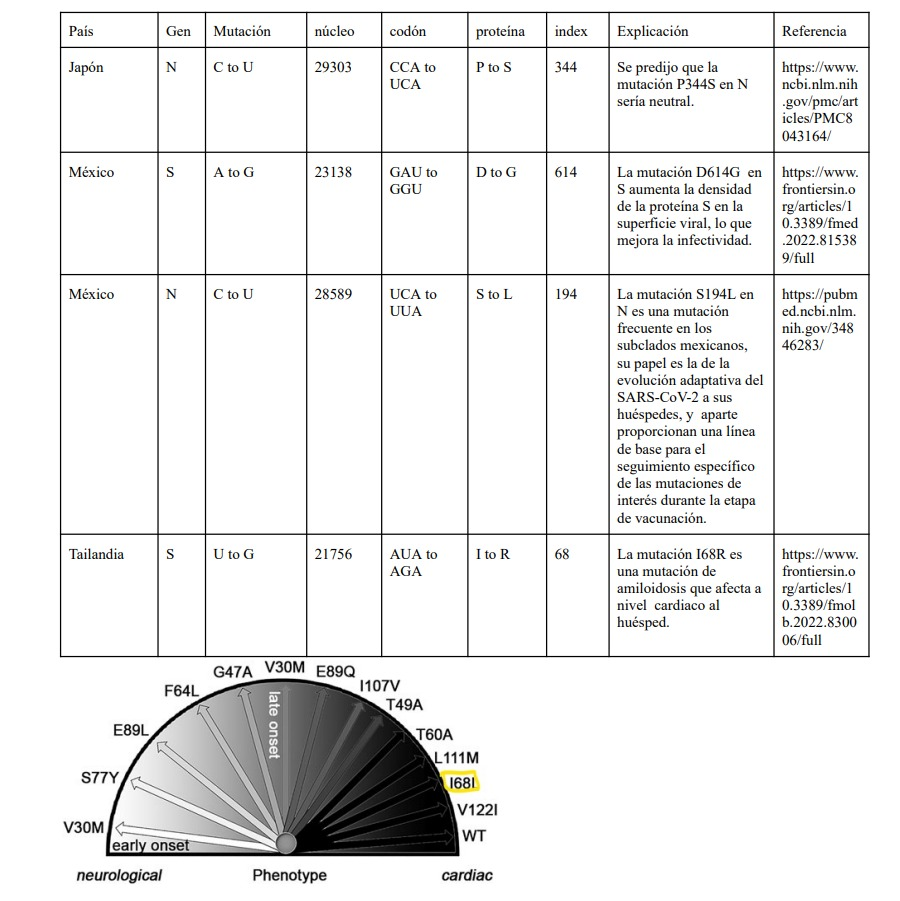
\includegraphics{Archivos/Image4.jpeg}

\hypertarget{conclusiones}{%
\subsubsection{Conclusiones:}\label{conclusiones}}

En conclusión, podemos observar que nuestras dos hipótesis son
correctas. Al analizar los primeros genomas de cada país, podemos ver
que no existen mutaciones en ellas. Las únicas mutaciones que vemos en
la tabla es una de Japón y dos de México. Tras nuestra investigación,
sabemos que la mutación de Japón no causa efectos en el virus. Para el
genoma de México es importante recordar que el virus llegó desde Italia,
no directamente de Wuhan, es por ello que vemos dos mutaciones
importantes que sí cambian al virus, especialmente en el aspecto de
infectividad como lo es para el caso de la mutación D614G. Esta mutación
fue de las primeras más importantes y permanentes en el virus ya que lo
volvió más fuerte. Todos los genomas actuales del virus contienen esta
mutación.

Por todo lo anterior, podemos establecer que prácticamente no hubo
mutaciones en los genes estructurales cuando el virus viajó directamente
de Wuhan a los otros países estudiados, la única excepción siendo Japón.
Además, podemos establecer una hipótesis para futuros análises la cual
es: ``El virus sufrió 2 o más mutaciones estructurales importantes al
viajar de un país secundario a uno terciario''.

Lamentablemente, no se puede concluir con certeza que nuestra segunda
hipótesis es correcta, ya que aunque sí podemos ver que dos meses
después sí hay más mutaciones, estas no son realmente significantes ni
sabemos si son lo suficientemente mortales para crear una variante. Para
determinar si las mutaciones encontradas tienen el poder de crear una
variante, sería necesario comparar los genomas con algunas variantes
conocidas como Alpha, Omicron y Delta. Sin embargo, sí pudimos observar
que en países que había llegado con mutaciones, dos meses después ya
tenían una o dos. Es interesante ver que aunque el virus se propaga muy
rápido, dos meses es un periodo de tiempo muy corto para realmente tener
una cantidad de mutaciones significante.

\hypertarget{datasets}{%
\subsubsection{Datasets:}\label{datasets}}

2019-12 - Genoma Original Wuhan:
\url{https://www.ncbi.nlm.nih.gov/nuccore/NC_045512}

2020-01-22 - Primer Genoma B Estados Unidos:
\url{https://www.ncbi.nlm.nih.gov/nuccore/MN994468} 2020-03-25 - Primer
Genoma B.1 México: \url{https://www.ncbi.nlm.nih.gov/nuccore/MT810786}
2020-01-30 - Primer Genoma B Italia:
\url{https://www.ncbi.nlm.nih.gov/nuccore/MT509662} 2020-01 - Primer
Genoma B Japón: \url{https://www.ncbi.nlm.nih.gov/nuccore/LC529905}
2020-01-08 - Primer Genoma B Tailandia:
\url{https://www.ncbi.nlm.nih.gov/nuccore/MT447155} 2020-03 - Primer
Genoma B Francia: \url{https://www.ncbi.nlm.nih.gov/nuccore/MT470129}

2020-03-30 - Genoma B Dos Meses Después Estados Unidos:
\url{https://www.ncbi.nlm.nih.gov/nuccore/MT772557} 2020-03-30 - Genoma
B.1 Dos Meses Después México:
\url{https://www.ncbi.nlm.nih.gov/nuccore/OK435602} 2020-03-23 - Genoma
B.1 Dos Meses Después Italia:
\url{https://www.ncbi.nlm.nih.gov/nuccore/MT509655} 2020-03 - Genoma B
Dos Meses Después Japón:
\url{https://www.ncbi.nlm.nih.gov/nuccore/LC542809} 2020-03-03 - Genoma
B Dos Meses Después Tailandia:
\url{https://www.ncbi.nlm.nih.gov/nuccore/MT781414} 2020-03 - Genoma B
Dos Meses Después Francia:
\url{https://www.ncbi.nlm.nih.gov/nuccore/MT470129}

2021-05-01 - Genoma A.2.5 México:
\url{https://www.ncbi.nlm.nih.gov/nuccore/ON316653} 2020-05-15 - Genoma
B.1 México: \url{https://www.ncbi.nlm.nih.gov/nuccore/OM000280}
2020-05-30 - Genoma B.1.595 México:
\url{https://www.ncbi.nlm.nih.gov/nuccore/OM181179}

\hypertarget{bibliografuxeda}{%
\subsubsection{Bibliografía:}\label{bibliografuxeda}}

Word Health Organization. (2020). WHO Statement regarding cluster of
pneumonia cases in Wuhan, China. Recuperado de:
\url{https://www.who.int/china/news/detail/09-01-2020-who-statement-regarding-cluster-of-pneumonia-cases-in-wuhan-china}

Word Health Organization. (2020). WHO Director-General's remarks at the
media briefing on 2019-nCoV on 11 February 2020. Recuperado de:
\url{https://www.who.int/dg/speeches/detail/who-director-general-s-remarks-at-the-media-briefing-on-2019-ncov-on-11-february-2020}

COVID-19: Problemas sociales y psicológicos en la pandemia. (2020, 16
diciembre). UNESCO. Recuperado 30 de abril de 2022, de
\url{https://es.unesco.org/news/covid-19-problemas-sociales-y-psicologicos-pandemia\#:\%7E:text=Ella\%20constituye\%20una\%20situaci\%C3\%B3n\%20disruptiva,de\%20bienes\%2C\%20o\%20del\%20empleo}.

Cronología de la respuesta de la OMS a la COVID-19‎. (2020, 29 junio).
Organización Mundial de la Salud. Recuperado 30 de abril de 2022, de
\url{https://www.who.int/es/news/item/29-06-2020-covidtimeline}

\end{document}
